% szablon sprawozdania z dnia 2020-10-27
\documentclass{article} % mwart , article
\usepackage[polish]{babel}
\usepackage[utf8]{inputenc}	
\usepackage{polski}	
\usepackage[T1]{fontenc}
\frenchspacing	
\usepackage{indentfirst}
% PAKIETY DO MODYFIKACJI SRONY
\usepackage{geometry}
\geometry{
	total={170mm,250mm},
	left=20mm,
	top=20mm,
}
% TABELA
\usepackage{multirow}
\usepackage{graphicx}
\usepackage{array}
\usepackage{makecell}
% INNE
\usepackage{color, colortbl}
\definecolor{Gray}{gray}{0.9}
\usepackage{lipsum}
% USTAWIENIA SUBSECTION
\usepackage[compact]{titlesec}
\titleformat{\subsection}[runin]
{\normalfont\large\bfseries}{\thesubsection}{1em}{}[{\\[0,5em]}]
\titlespacing*{\subsection}{1cm}{1em}{0em}
% dodanie FORCEINDENT
\newcommand{\forceindent}{\leavevmode{\parindent=1cm\indent}} %


% TYTUŁ, DATY ORAZ DANE OSOBY OPRACOWUJĄCEJ SPRAWOZDANIE
\def\AuthorFirstName{MARCIN}
\def\AuthorLastName{KOWOL}
\def\Title{Lab 4 -  zastosowane poleceń GIT}
\def\DateOfExecution{2023-10-25}
\def\DateOfDeliver{2023-11-06}
%
%
\begin{document}
\noindent
\def\arraystretch{1.5} \small
% TABELA Z DANYMI
\begin{table}
    \resizebox{\textwidth}{!}{\begin{tabular}{|p{2cm}|p{4cm}|p{3cm}|p{3cm}|l|}
            \hline
            \multirow{4}{*}{\makecell[l]{
\includegraphics[width=2cm]{image/ModLogoPO}                                                                                                                                      \\
\includegraphics[width=2cm]{image/ModLogoWE}}} & PRZEDMIOT: & \multicolumn{3}{l|}{ \makecell[l]{\noalign{\vskip3pt}PRZEDMIOT WYBIERALNY XIV:\\ NARZ\k{E}DZIA INFORMATYCZNE W PRAKTYCE \\IN\.{Z}YNIERSKIEJ}}\tabularnewline
            \cline{2-5} \cline{3-5} \cline{4-5} \cline{5-5}
                      & KIERUNEK STUDIÓW:                                                                     & INFORMATYKA                                         & ROK STUDIÓW:                     & IV\tabularnewline
            \cline{2-5} \cline{3-5} \cline{4-5} \cline{5-5}
                      & ROK AKADEMISKI:                                                                       & 2020/2021                                           & SEMESTR:                         & 7\tabularnewline
            \cline{2-5} \cline{3-5} \cline{4-5} \cline{5-5}
                      & TEMAT:  \multicolumn{3}{l|}{\makecell[l]{\noalign{\vskip3pt} \Title }}\tabularnewline
            \hline
            IMI\k{E}: & \textbf{\AuthorFirstName}                                                             & \multicolumn{2}{l|}{DATA WYKONANIA \'{C}WICZENIA: } & \DateOfExecution \tabularnewline
            \hline
            NAZWISKO: & \textbf{\AuthorLastName}                                                              & \multicolumn{2}{l|}{DATA ODDANIA SPRAWOZDANIA:}     & \DateOfDeliver \tabularnewline
            \hline
            OCENA:    & DATA:                                                                                 & \multicolumn{3}{l|}{UWAGI}\tabularnewline
            \hline \rowcolor{Gray}
            {\makecell[l]{                                                                                                                                                                                                 \\ \\ \\ \\}}&  & \multicolumn{3}{l|}{}\tabularnewline
            \hline
        \end{tabular}}
\end{table}
% POCZĄTEK SPRAWOZDANIA

\section{Zadanie 4 z zajęć laboratoryjnych}
\subsection{GIT CONFIG}
\forceindent git config --list

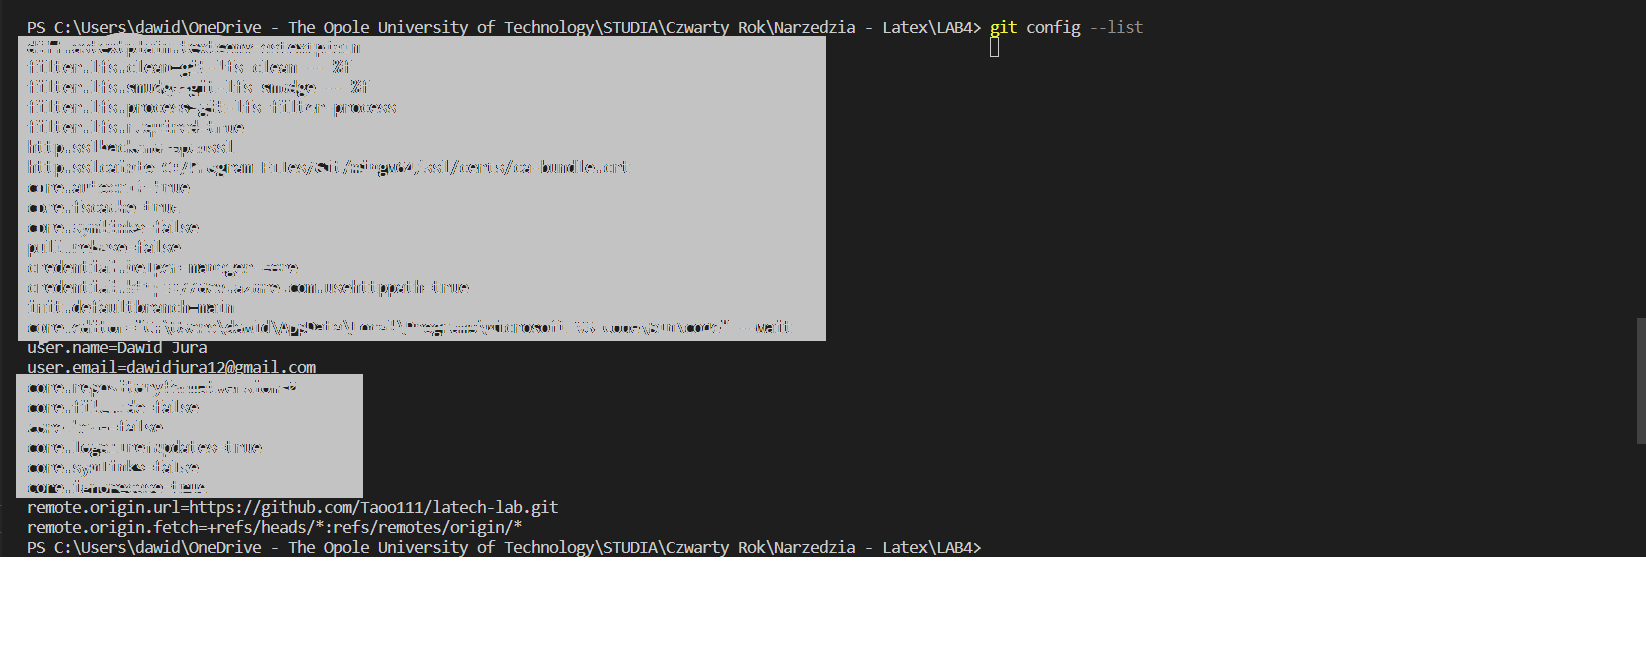
\includegraphics[width=18cm]{image/config.png}
\subsection{GIT INIT}
\forceindent git init

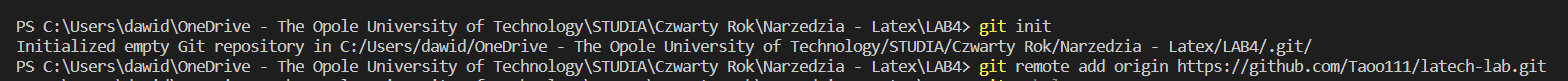
\includegraphics[width=18cm]{image/init.png}
\subsection{GIT STATUS}
\forceindent git status

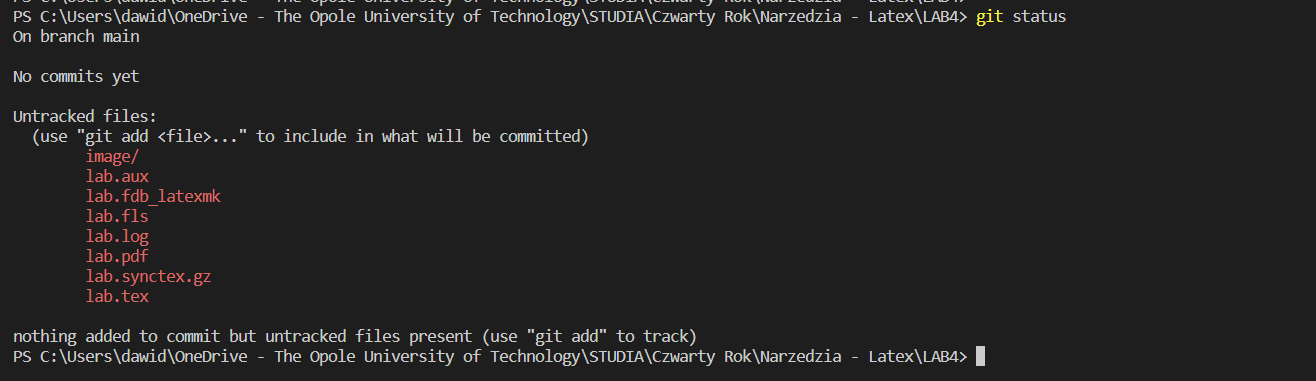
\includegraphics[width=18cm]{image/status.png}
\subsection{GIT ADD}
\forceindent git add -A

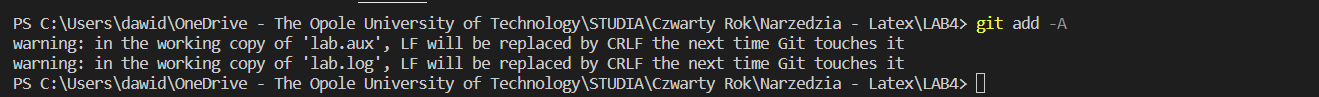
\includegraphics[width=18cm]{image/add.png}
\subsection{GIT COMMIT}
\forceindent git commit -m "first files"

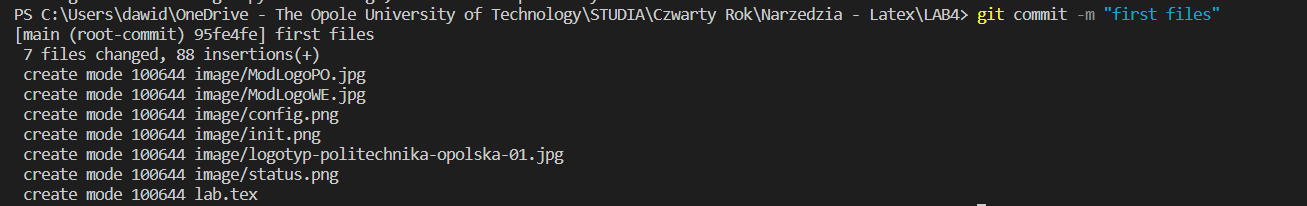
\includegraphics[width=18cm]{image/commit.png}
\subsection{GIT DIFF}
\forceindent git diff

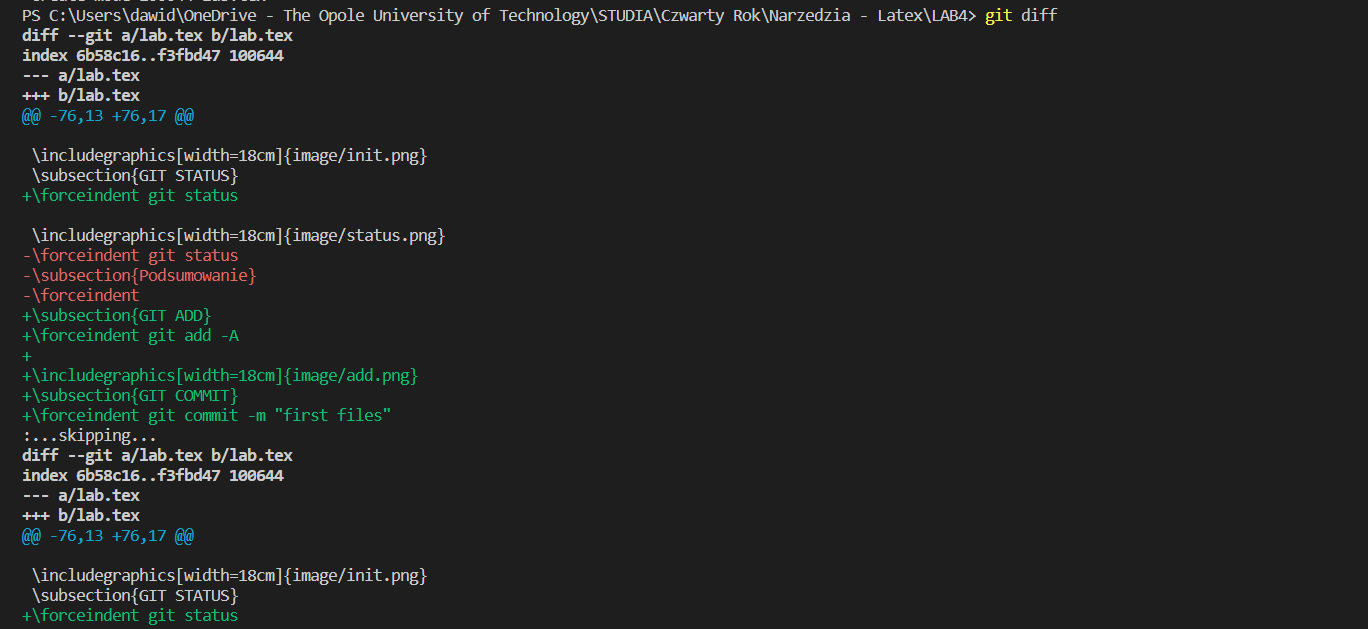
\includegraphics[width=18cm]{image/diff.png}
\subsection{GIT BRANCH}
\forceindent git branch

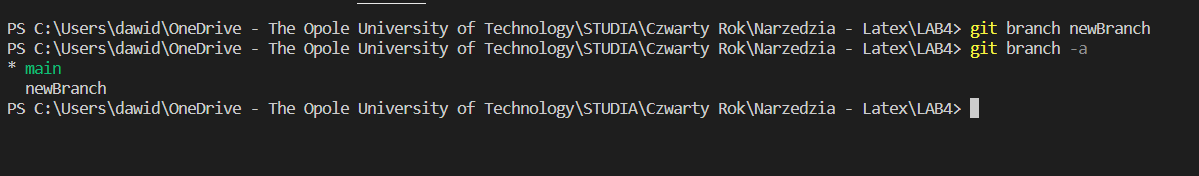
\includegraphics[width=18cm]{image/branch.png}
\subsection{GIT CHECKOUT}
\forceindent git checkout

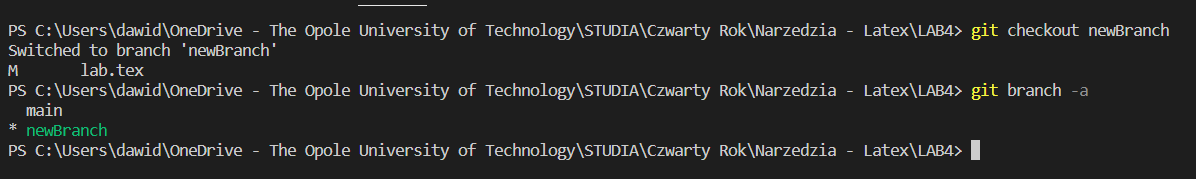
\includegraphics[width=18cm]{image/checkout.png}
\subsection{GIT MERGE}
\forceindent git merge

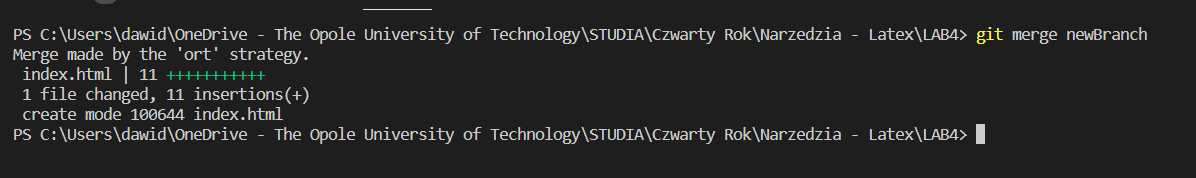
\includegraphics[width=18cm]{image/merge.png}
\subsection{GIT RESTORE}
\forceindent git restore -> przywracanie zawartości plików w katalogu roboczym do ich stanu z ostatniego zatwierdzonego commita

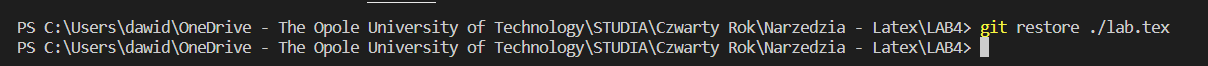
\includegraphics[width=18cm]{image/restore.png}
\subsection{GIT RM}
\forceindent git rm

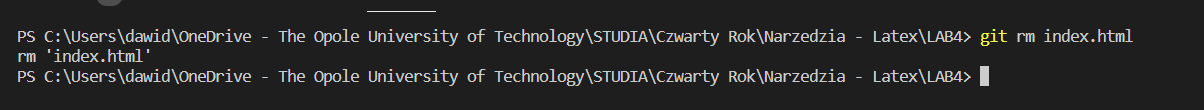
\includegraphics[width=18cm]{image/rm.png}

\end{document}